\documentclass[12pt]{article}

% packages

\usepackage{blindtext}

\usepackage[utf8]{inputenc}
\usepackage[T1]{fontenc}
\usepackage[english, ngerman]{babel}

\usepackage[top=30mm, bottom=30mm, left=20mm, right=20mm]{geometry}
\usepackage{fancyhdr}
\usepackage{setspace}
\usepackage{parskip}

\usepackage{graphicx}
\usepackage[section]{placeins}
\usepackage[table, dvipsnames]{xcolor}
\usepackage{pdfpages}

\usepackage{hyperref}
\usepackage[labelfont=bf]{caption}

\usepackage[round]{natbib}

\usepackage{listings}
\usepackage{minted}
\usepackage{algorithmicx}
\usepackage[noend]{algpseudocode}
\usepackage{algorithm}

\usepackage{tabularx}
\usepackage{multirow}
\usepackage{multicol}
\usepackage{caption}
\usepackage{subcaption}
\usepackage{adjustbox}

\usepackage{amsmath}

%%%%%%%%%%%%%%%%%%%%%% preamble %%%%%%%%%%%%%%%%%%%%%%

\renewcommand*{\sectionmark}[1]{ \markright{\thesection\ ##1} }
% \renewcommand*{\chaptermark}[1]{ \markboth{\chaptername\ \thechapter: ##1}{} }
\fancyhead[LE,RO]{\thepage}
\fancyhead[LO,RE]{}
\fancyfoot{}
\pagestyle{fancy}

\definecolor{myblue}{RGB}{46, 59, 160}

\graphicspath{{pics/}}

\hypersetup{
	pdfstartpage=7,
    pdfstartview = FitB,
	pdfpagelayout=SinglePage,
	pdftitle={PC1-Projektarbeit},
	pdfsubject={PC1-Projektarbeit},
	pdfauthor={Maurice Wenig},
	pdfcreator={Maurice Wenig},
	pdfproducer={Maurice Wenig},
	pdfkeywords={meta, information, pdf, hyperref, latex},
	colorlinks=true,
	linkcolor=myblue,
	citecolor=myblue
}

\bibliographystyle{unsrtnat}

\newcommand*\justify{%
  \hyphenchar\font=`\-% allowing hyphenation
}

\definecolor{line_number_colour}{rgb}{0.5,0.5,0.5}
\renewcommand\theFancyVerbLine{\color{line_number_colour}\tiny\arabic{FancyVerbLine}}
\setminted[C]{
	% linenos, 
	breaklines,
	fontsize=\footnotesize
}

\hyphenpenalty=5000
\tolerance=5000

% TODO: remove for digital version
% \selectcolormodel{gray}

%%%%%%%%%%%%%%%%%%%%%% main %%%%%%%%%%%%%%%%%%%%%%

\begin{document}

\thispagestyle{empty}
\begin{center}
    \begin{LARGE}
        \textbf{Projektarbeit PC1}
    \end{LARGE}\vspace{3mm}\\
    \begin{Large}
        \textbf{Dokumentation}
    \end{Large}\vspace{5mm}\\
    \begin{large}
        Maurice Wenig
    \end{large}
\end{center}
% \setcounter{tocdepth}{1}
\tableofcontents
\clearpage

% \input{chapters/Kurzfassung.tex}
% im Anschluss an das Inhaltsverzeichnis gegebenenfalls ein Verzeichnis der Symbole (oder Abkürzungen u. ä.) anfügen.

\fancyhead[LO,RE]{\itshape\nouppercase\leftmark}
\section{Vorgehen}
Das initiale Feld wird gleichmäßig auf alle Prozesse aufgeteilt. In jedem Prozess werden die neuen Temperaturen im lokalen $chunk$ berechnet. Dafür gibt es einen Austausch der aktuellen Werte mit den Nachbarprozessen. Diese Werte werden in den Ghost Cells in einem Halo der Breite $g$ um den lokalen $chunk$ gespeichert.
Ab hier werden die Ghost Cells als Teil des lokalen Chunks angesehen. Der Teil des Chunks, der keine Ghost Cells beinhaltet, wird als innerer Chunk bezeichnet.
Am Ende der Berechnung werden die innneren Chunks der einzelnen Prozesse wieder zusammengesetzt.

\begin{algorithmic}[1]
    \State split\_up\_domain()
    \For{$i = 0 \rightarrow n\_iterations$}
        \If{$i \% g == 0$}
            \State exchange\_ghost\_cells()
        \EndIf
        \State calculate()
    \EndFor
    \State collect()
\end{algorithmic}
\subsection{Kommunikation}
Die angewandten Techniken werden größtenteils dem Paper ``Ghost Cell Pattern'' von \citeauthor{Kjolstad2010} entnommen.
Es wird ein Deep Halo benutzt und die Corner Cells sollen auch effizient übertragen werden.
Da die Ost-West-Kommunikation immer vor der Nord-Süd-Kommunikation passieren muss, damit die Ecken richtig übertragen werden, wird zwischen der Kommunikation von den beiden Richtungen gewartet.

\begin{algorithmic}[1]
    \State irecv\_east()
    \State irecv\_west()
    \State isend\_east()
    \State isend\_west()
    \State wait()
    \State irecv\_north()
    \State irecv\_south()
    \State isend\_north()
    \State isend\_south()
    \State wait()
\end{algorithmic}

Falls ein Nachbar in eine Richtung nicht existiert, werden die Ghost Cells mit Padding gefüllt. Dabei wird immer der nächste Wert des inneren Chunks kopiert.

\subsection{Berechnung}
Es werden immer nur so viele Zellen berechnet, wie für den nächsten Schritt benötigt werden. Dafür wird eine $border$ eingeführt.
Am Anfang umfasst die $border$ den ganzen Chunk, inklusive Halo, bis auf den äußersten Ring. Am Ende umfasst die $border$ nur noch den inneren Chunk.
% TODO: fancy visualisation

Um die neuen Werte zu berechnen werden zwei Arrays benutzt. Eines, das die alten Werte enthält und eines, das die Ergebnisse der Berechnung enthält. Als Vorbereitung für den nächsten Schritt werden am Ende der Berechnung die Arrays vertauscht.

\begin{algorithmic}[1]
    \State $border$ := adapt\_border()
    \For{$x,y$ in the $border$}
        \State results[$x,y$] := calculation\_step($x,y$) \Comment{calculation\_step uses old\_values}
    \EndFor
    \State swap(results, old\_values)
\end{algorithmic}


\clearpage
\section{Implementierung}
% TODO: update lines
\subsection{Chunks}
Zu dem inneren Chunk kommt noch das Ghost-Block-Halo dazu:
\inputminted[fontsize=\scriptsize, firstline=73, lastline=78]{C}{../src/waermeleitung.cpp}

\subsection{Kommunikation}
\subsubsection{Ghost Cells}
Für bessere Lesbarkeit werden die Axen \verb+X_AXIS,Y_AXIS+ und die Richtungen \verb+EAST,WEST,NORTH,SOUTH+ definiert. Den Richtungen werden relative Positionen im Gitter zugewiesen. Außerdem werden ein \verb+MAIN_RANK+ definiert, der alles sammelt und ausgibt, sowie ein undefinierter Rang \verb+UNDEFINED_RANK+, der für Nachbarn außerhalb des Gitters steht.
\inputminted[fontsize=\scriptsize, firstline=31, lastline=57]{C}{../src/waermeleitung.h}
Um die Blöcke von Ghost Cells effizient zu verschicken, werden Vektoren von MPI verwendet.
\inputminted[fontsize=\scriptsize, firstline=60, lastline=71]{C}{../src/waermeleitung.cpp}
\inputminted[fontsize=\scriptsize, firstline=3, lastline=16]{C}{../src/comms.cpp}
Die Punkte, an denen Blöcke anfangen, werden hier definiert:
\inputminted[fontsize=\scriptsize, firstline=18, lastline=29]{C}{../src/comms.cpp}
Mit \verb+neighbours[direction]+ als Rang des Nachbars in der jeweiligen Richtung wird dann wie folgt kommuniziert:
\inputminted[fontsize=\scriptsize, firstline=59, lastline=80]{C}{../src/comms.cpp}
Padding:
\inputminted[fontsize=\scriptsize, firstline=31, lastline=57]{C}{../src/comms.cpp}
\subsubsection{Collect}
Die inneren Chunks werden dann konzentriert hintereinander in einen Buffer geschrieben. Die Werte im Buffer werden für das Ergebnis umgeordnet.
\inputminted[fontsize=\scriptsize, firstline=44, lastline=48]{C}{../src/print.cpp}

\subsection{Berechnung}
Berechnung nach Aufgabenstellung mit \verb+FACTOR+ $= \alpha \cdot \frac{\Delta t}{h^2}$.
\inputminted[fontsize=\scriptsize, firstline=135, lastline=142]{C}{../src/waermeleitung.cpp}


\clearpage
\section{Benutzung}
Argumente, die übergeben werden müssen:
\begin{itemize}
    \item Größe des zu berechnenden Feldes
    \item Anzahl der Iterationen
    \item Anzahl der Prozesse in X-Richtung
    \item Anzahl der Prozesse in Y-Richtung
\end{itemize}
Parameter, die angepasst werden können:
\begin{itemize}
    \item Ausgabedatei
    \item Breite des Ghost Cell Halos
    \item Abstand der Iterationen, in denen ein Zwischenstand gespeichert wird
\end{itemize}

\clearpage
\section{Auswertung}
(Disclaimer:) Die Performance wurde auf meinem lokalen Rechner gemessen, da es auf dem ARA-Cluster zu fehlern kam (siehe \verb+README.md+).

\begin{figure}[!htb]
    \begin{subfigure}{0.5\textwidth}
        \centering
        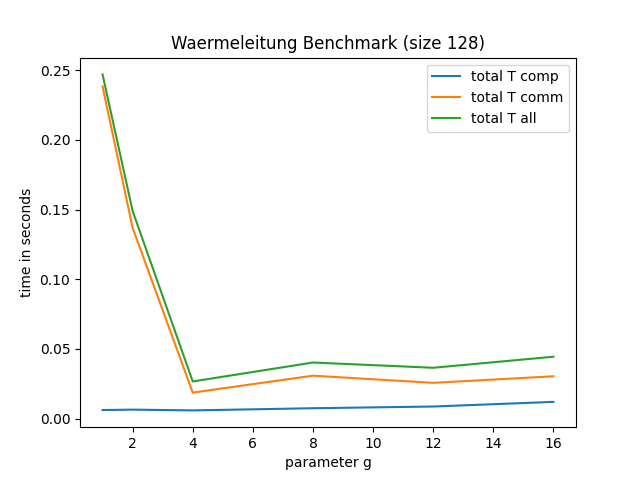
\includegraphics[scale=0.5]{../benchmark/plots/plot_total_128.png}
        \caption{field size 128}\label{fig:plot_128_tot}
    \end{subfigure}
	\begin{subfigure}{0.5\textwidth}
        \centering
        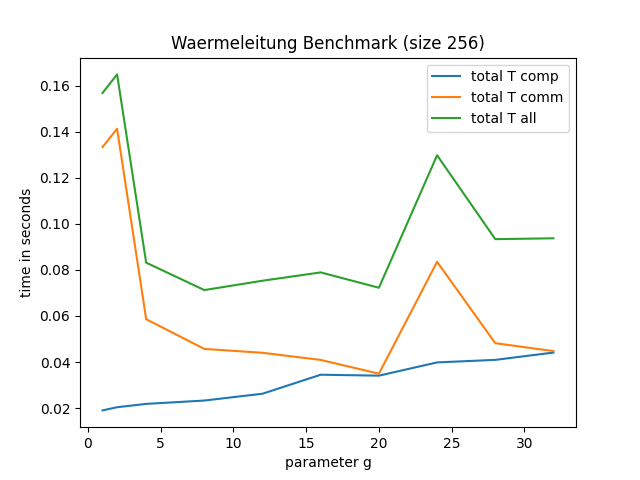
\includegraphics[scale=0.5]{../benchmark/plots/plot_total_256.png}
        \caption{field size 256}\label{fig:plot_256_tot}
    \end{subfigure}
    \newline
    \begin{subfigure}{0.5\textwidth}
        \centering
        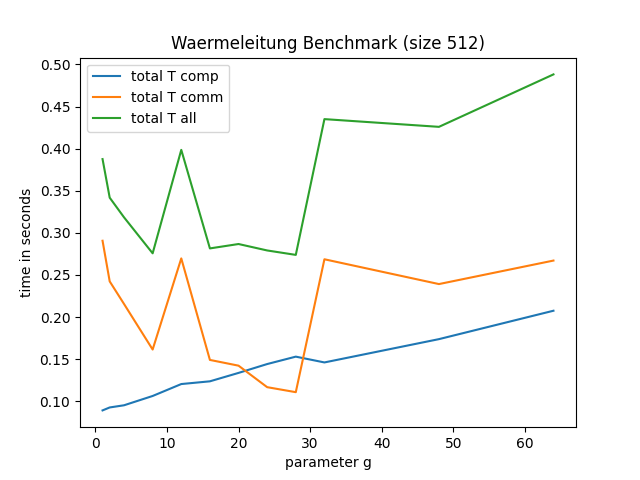
\includegraphics[scale=0.5]{../benchmark/plots/plot_total_512.png}
        \caption{field size 512}\label{fig:plot_512_tot}
    \end{subfigure}
	\begin{subfigure}{0.5\textwidth}
        \centering
        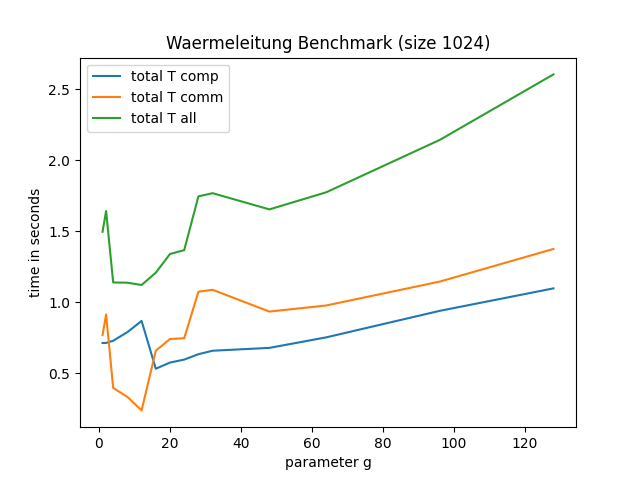
\includegraphics[scale=0.5]{../benchmark/plots/plot_total_1024.png}
        \caption{field size 1024}\label{fig:plot_1024_tot}
    \end{subfigure}
    \begin{center}
        \begin{subfigure}{0.5\textwidth}
            \centering
            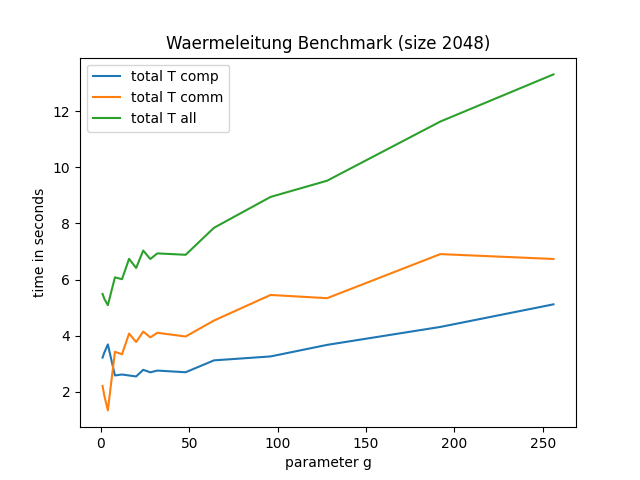
\includegraphics[scale=0.5]{../benchmark/plots/plot_total_2048.png}
            \caption{field size 2048}\label{fig:plot_2048_tot}
        \end{subfigure}
    \end{center}
	\caption{Zeitverteilung gesamt}
    \label{fig:all_time}
\end{figure}

\begin{figure}[!htb]
    \begin{subfigure}{0.5\textwidth}
        \centering
        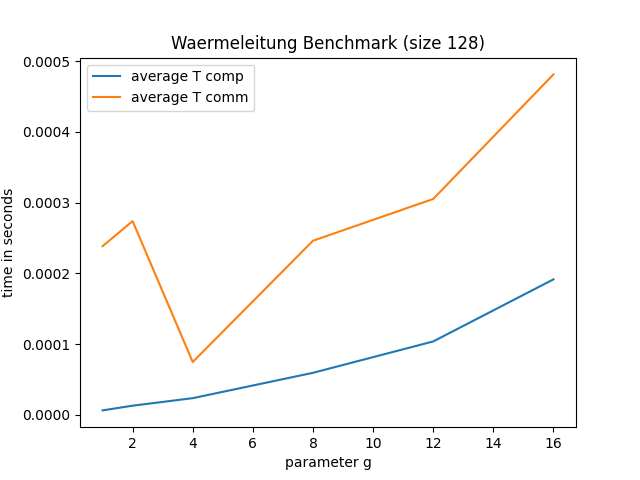
\includegraphics[scale=0.5]{../benchmark/plots/plot_avg_128.png}
        \caption{field size 128}\label{fig:plot_128_avg}
    \end{subfigure}
	\begin{subfigure}{0.5\textwidth}
        \centering
        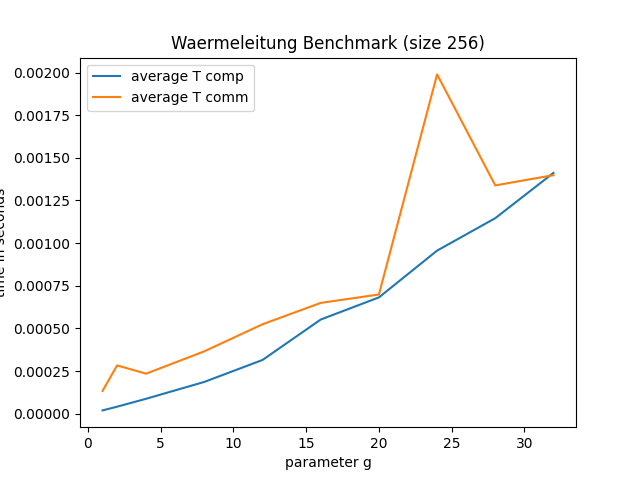
\includegraphics[scale=0.5]{../benchmark/plots/plot_avg_256.png}
        \caption{field size 256}\label{fig:plot_256_avg}
    \end{subfigure}
    \newline
    \begin{subfigure}{0.5\textwidth}
        \centering
        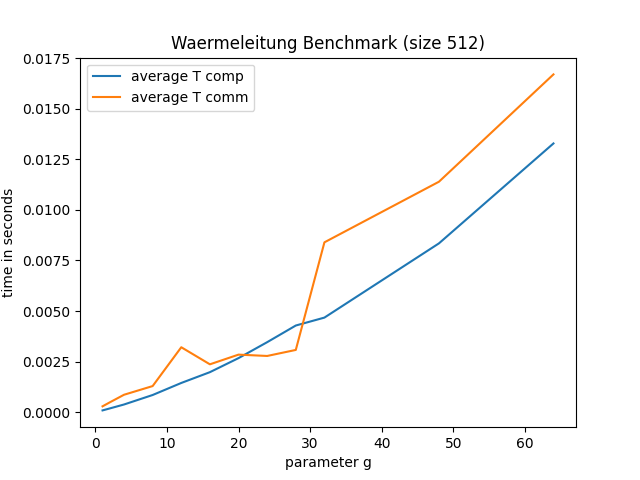
\includegraphics[scale=0.5]{../benchmark/plots/plot_avg_512.png}
        \caption{field size 512}\label{fig:plot_512_avg}
    \end{subfigure}
	\begin{subfigure}{0.5\textwidth}
        \centering
        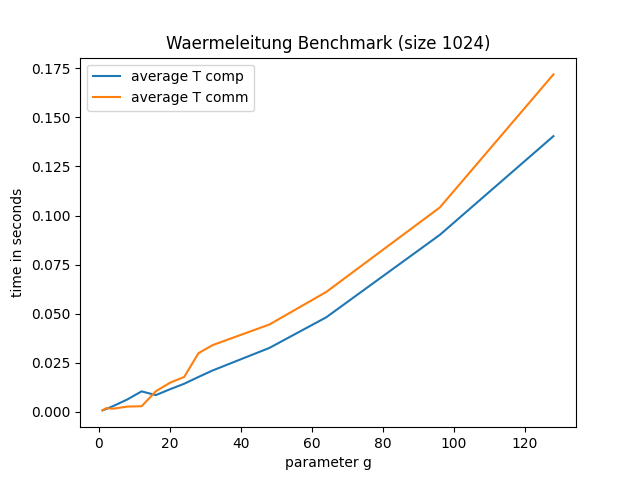
\includegraphics[scale=0.5]{../benchmark/plots/plot_avg_1024.png}
        \caption{field size 1024}\label{fig:plot_1024_avg}
    \end{subfigure}
    \begin{center}
        \begin{subfigure}{0.5\textwidth}
            \centering
            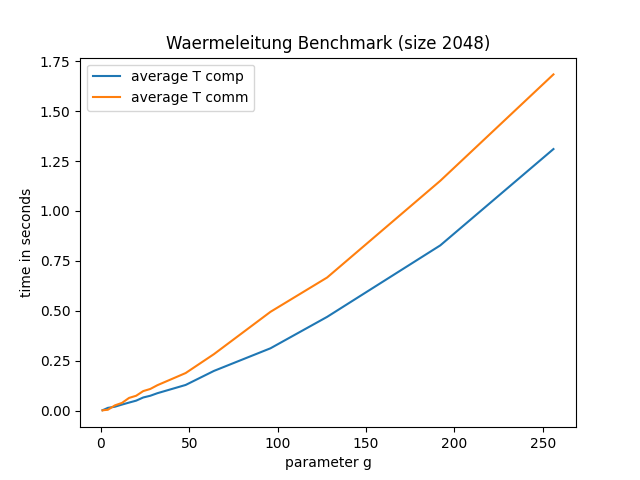
\includegraphics[scale=0.5]{../benchmark/plots/plot_avg_2048.png}
            \caption{field size 2048}\label{fig:plot_2048_avg}
        \end{subfigure}
    \end{center}
	\caption{Zeitverteilung einzelner Zeitschritt}
    \label{fig:single_time}
\end{figure}

Jeder Prozess hat einzeln die Zeiten der Berechnungs- und Kommunikationszeiten für einzelne Schritte gemessen. Daraus wurden Gesamtzeiten und Durchschnittszeiten der einzelnen Prozesse berechnet. Über den Prozessen wurde dann der Durchschnitt gezogen.
Die Gesamtzeit des Programms wurde nur vom main rank gemessen.

Wie man in \autoref{fig:all_time} sieht, führt eine Erhöhung der Halobreite zuerst zu einer Verbesserung der Laufzeit, da der Aufbau der Kommunikation deutlich länger braucht als die Berechnung der inneren Werte. 
Durch höhere Halobreite wird seltener kommuniziert und mehr berechnet. 
Die zusätzliche Menge an übertragenen Daten sind erst nicht relevant, da der Kommunikationsaufbau länger braucht als die tatsächliche Übertragung der Daten.

Die höhere Halobreite führt später allerdings zu einer Verlangsamung.
In \autoref{fig:single_time} ist gut zu sehen, dass die Kommunikationszeiten schneller steigen als die Berechnungszeiten.
Die Vermutung ist, dass ab dieser Halobreite die Übertragung länger dauert, als der Aufbau der Kommunikation.
Die zunehmende Redundanz der Berechnungen ist sicherlich auch ein Grund für die Verlangsamung.

Die Berechnung wäre sicherlich noch um einiges schneller, wenn die Kommunikation während der Berechnung ablaufen würde, und nicht nur halb-asynchron und vor der Berechnung.
\FloatBarrier

\typeout{}
\clearpage
\pagestyle{empty}
\bibliography{literatur}
% \listoffigures
% \listoftables
% \appendix
% \input{chapters/Anhang}

\end{document}